\documentclass[12pt,a4paper]{article}

%% ─── Packages ────────────────────────────────────────────────────────────────
\usepackage[top=1in,bottom=1in,left=1.1in,right=1.1in]{geometry}
\usepackage{amsmath,amssymb}
\usepackage[hidelinks]{hyperref}
\usepackage{enumitem}
\usepackage{xcolor}
\usepackage{float}
\usepackage{tikz}
\usetikzlibrary{arrows.meta,positioning,shapes.geometric,calc}
\usepackage{setspace}
\usepackage{parskip}
\usepackage{titlesec}
\usepackage{microtype}
\usepackage{graphicx}
\usepackage{booktabs}
\usepackage{array}
\usepackage{fancyhdr}

%% ─── Spacing ─────────────────────────────────────────────────────────────────
\onehalfspacing
\setlength{\parindent}{0pt}
\setlength{\parskip}{0.65em}

%% ─── Colours ─────────────────────────────────────────────────────────────────
\definecolor{mainblue}{RGB}{25,95,175}
\definecolor{lightblue}{RGB}{218,232,252}
\definecolor{darkgray}{RGB}{60,60,60}
\definecolor{arrowgray}{RGB}{110,110,110}
\definecolor{nodered}{RGB}{190,50,30}
\definecolor{nodegreen}{RGB}{30,140,80}
\definecolor{lightyellow}{RGB}{255,250,220}
\definecolor{lightgreen}{RGB}{220,248,230}

%% ─── Section headings ────────────────────────────────────────────────────────
\titleformat{\section}
  {\large\bfseries\color{mainblue}}
  {\thesection.}{0.55em}{}
  [\vspace{0.1em}{\color{mainblue!50}\rule{\linewidth}{0.6pt}}]

\titleformat{\subsection}
  {\normalsize\bfseries\color{darkgray}}
  {\thesubsection}{0.6em}{}

\titlespacing*{\section}{0pt}{1.6em}{0.6em}
\titlespacing*{\subsection}{0pt}{1em}{0.3em}

%% ─── Header / footer ─────────────────────────────────────────────────────────
\pagestyle{fancy}
\fancyhf{}
\renewcommand{\headrulewidth}{0.3pt}
\fancyhead[L]{\small\color{darkgray} Knowledge-Graph-Driven Multilingual Educational Platform}
\fancyhead[R]{\small\color{darkgray} BTP Report · IIIT Hyderabad}
\fancyfoot[C]{\thepage}


%% ═══════════════════════════════════════════════════════════════════════════
\begin{document}
\thispagestyle{empty}

%% ─── Title Page ─────────────────────────────────────────────────────────────
\begin{center}
\vspace*{1.2cm}
{\large\bfseries International Institute of Information Technology, Hyderabad}\\[0.25cm]
{\normalsize Department of Computer Science and Engineering}\\[1.4cm]

{\color{mainblue}\rule{\linewidth}{1.8pt}}\\[0.8cm]

{\LARGE\bfseries A Knowledge-Graph-Driven\\[0.45cm]
Multilingual Educational Platform\\[0.45cm]
for Indian School Curricula}\\[0.8cm]

{\color{mainblue}\rule{\linewidth}{1.8pt}}\\[2.2cm]

{\large B.Tech Thesis Project (BTP)}\\[0.35cm]
{\large Academic Year 2025--2026}\\[2.6cm]

\renewcommand{\arraystretch}{1.9}
\begin{tabular}{c@{\qquad\qquad\quad}c}
  \textbf{\large Saksham Chitkara} & \textbf{\large Swam Singla} \\
  {\normalsize Roll No.\ 2023101021} & {\normalsize Roll No.\ 2023101134}
\end{tabular}

\vfill
{\large May 2026}
\end{center}

\newpage
\thispagestyle{plain}

%% ─── Abstract ────────────────────────────────────────────────────────────────
\begin{abstract}
\noindent
India has over 250 million school students, the vast majority of whom learn in regional
languages rather than English.
Yet high-quality, curriculum-aligned educational content in Indic languages is almost
entirely absent from digital platforms.
This project builds a multilingual educational platform for school Mathematics and Science,
covering Grades~6 through~12 across NCERT, ICSE, and several state boards.

The project evolved through two major phases.
The first phase extracted sections directly from official textbook PDFs,
generated explanations using a locally hosted language model,
and translated them into Hindi, Telugu, and Odia through a neural translation pipeline.
This produced working results but revealed a deep structural flaw: organising content
by textbook chapter rather than by concept led to inconsistency, redundant generation,
broken translation of mathematical notation, and no meaningful navigation between related ideas.

The second phase rebuilt the system from the ground up around a \emph{knowledge graph}:
a directed network of canonical concepts linked by prerequisite relationships.
Every concept is defined and generated exactly once.
Content is grounded in the original textbooks through Retrieval-Augmented Generation (RAG),
and produced directly in all four languages using Sarvam~AI models,
eliminating the translation step entirely.
The result is a web platform where any concept in the curriculum (from Whole Numbers in
Grade~6 to Differential Equations in Grade~12) is one click away from everything the
student needs to know before it and everything it enables next.
\end{abstract}

\tableofcontents
\newpage

%% ═══════════════════════════════════════════════════════════════════════════
\section{Introduction}

India runs one of the largest school education systems in the world,
with hundreds of millions of students across thousands of schools.
Yet the digital resources available to those students are almost entirely in English,
and high-quality regional language content for school Mathematics and Science is largely absent.

The existing digital landscape for school education presents a consistent set of limitations:

\begin{itemize}[leftmargin=2em, itemsep=0.3em]
  \item Most free content available online is in English. Regional language material,
    where it exists, is typically a translation of English source text rather than content
    written natively for the regional language learner.
  \item Official digital platforms that put textbooks online retain the same linear,
    chapter-based organisation as the printed book. There is no concept navigation,
    no links between related topics across chapters, and no way for a student to identify
    which foundational idea they are missing.
  \item Paid platforms are typically designed for competitive examination preparation.
    They are expensive, examination-focused rather than concept-focused,
    and regional language support beyond Hindi is limited.
  \item Free international platforms offer better concept structure and prerequisite maps,
    but are built around foreign curricula and are not well aligned with Indian boards.
\end{itemize}

The gap this project fills is specific: a free, multi-board educational platform covering
Mathematics and Science for Grades~6 through~12, structured around the actual relationships
between concepts, with content that a student can read in their own language and that
genuinely builds from what they already know toward what they are trying to learn.

This report describes the complete development of that platform: the first version,
what went wrong with it, the redesign it led to, and the system that resulted.

%% ═══════════════════════════════════════════════════════════════════════════
\section{Phase~1: The Chapter-Based Pipeline}

\subsection{Overview}

The first version of the system was designed around the most natural available structure:
the textbook itself.
NCERT books are organised into chapters, chapters into numbered sections,
and sections into content.
The pipeline followed this structure exactly: extract each section from the PDF,
generate an explanation, translate it, and serve it.

This produced a working product reasonably quickly,
but examining the output carefully revealed problems that were not bugs to be fixed;
they were consequences of the design.

\subsection{Extracting Structure from Textbook PDFs}

PDF files do not record semantic information.
They store drawing instructions: where to place which characters in which font.
Identifying headings versus body text therefore requires inferring structure from visual cues.

The heading extractor took a negation approach.
It first identified the dominant font across each document (the body text),
then treated any text in a substantially different, larger, or bolder font as a candidate heading.
This method handles inconsistent typography across grade levels without hardcoding
formatting rules for each individual textbook.

Extracted headings were assembled into a structured representation of each chapter's
section hierarchy for all subjects and grades.
This hierarchy became the skeleton that the rest of the pipeline operated on.

\subsection{Generating Explanations with a Language Model}

All language model inference in this project runs locally on a single consumer-grade GPU
with 4~GB of video memory.
This is a binding hardware constraint: large language models require far more memory unless
their numerical precision is aggressively reduced.

The technique used is \emph{4-bit quantisation}, which compresses model weights to
4-bit integer representation (roughly eight times smaller than the default 32-bit format),
at a modest cost in generation quality.
The model used was Meta's LLaMA~3.2~3B Instruct, quantised in NF4 format using the
BitsAndBytes library, occupying approximately 2~GB of video memory and leaving headroom
for inference.

Before generating a full explanation for a section,
the model first scored the section's importance on a scale of one to five.
This score determined the depth of content generated:
introductory sections received brief summaries while core concepts
received comprehensive explanations with multiple worked examples.
The actual textbook text for the section was provided to the model as context,
keeping the generated content grounded in the curriculum.

The tone and depth were calibrated to grade level.
For Grades~6 to~8, the prompt requested friendly, accessible language with everyday
analogies and encouragement.
For Grades~9 and~10, it requested a balance of accessibility and mathematical precision.
For Grades~11 and~12, it requested rigorous treatment appropriate for students
preparing for national-level university entrance examinations.

Each page followed a consistent structure: an introduction, a main explanation with
worked examples and formatted mathematical expressions, a section on common mistakes,
and a summary.
All mathematical notation was written in standard \LaTeX{} format so it could be rendered
as properly typeset symbols in the browser, for example, the quadratic formula as
$x = \dfrac{-b \pm \sqrt{b^2 - 4ac}}{2a}$ rather than a plaintext approximation.

\subsection{Translating into Regional Languages}

Generated English content was then translated into Hindi, Telugu, and Odia.
Three translation model families were implemented, compared, and made available
for selection.

\medskip
\noindent\textbf{IndicTrans2 (AI4Bharat)} is the current state-of-the-art model for
English-to-Indic translation, supporting all 22 scheduled Indian languages.
It runs locally in 16-bit floating-point precision at roughly 2~GB of video memory.
It produced the most fluent results for Hindi and Telugu.

\medskip
\noindent\textbf{Sarvam Translate (Sarvam AI)} is built on Google's Gemma~3 architecture
and produced particularly natural Hindi output with good handling of educational context.

\medskip
\noindent\textbf{TranslateGemma (Google)} is a translation-focused 4-billion-parameter model
run in 4-bit quantised form.
It was competitive for Hindi but produced weaker results for Odia.

\medskip
The most technically challenging aspect of the translation pipeline was preserving
mathematical notation.
If a sentence containing a \LaTeX{} formula is sent to a neural translation model,
the model treats the markup as text and typically corrupts, partially translates,
or removes it.
The solution was to split each sentence at formula boundaries before translation:
text segments were sent to the model, and \LaTeX{} expressions were passed through
untouched on a separate path.
After translation, the segments were reassembled.
This preserved mathematical content correctly in the large majority of cases.

A significant compatibility problem emerged with IndicTrans2.
It requires version~4.45 or older of the underlying HuggingFace Transformers library,
while the Sarvam model requires a newer version.
Critically, running IndicTrans2 on an incompatible version does not produce an error;
it silently generates completely garbled, unreadable output.
Diagnosing this took considerable time.
The two models could not share the same software environment,
requiring separate configurations to be maintained.

Generated and translated content was stored in a cloud-hosted database.
The web application served this content at addresses structured as
Grade $\rightarrow$ Subject $\rightarrow$ Chapter $\rightarrow$ Section.

\subsection{Problems Identified}

After running the full pipeline and examining the output systematically,
several fundamental problems became clear.
These were not implementation bugs; they were direct consequences of the chapter-based design.

\medskip
\noindent\textbf{The same concept was generated multiple times, inconsistently.}
Mathematical concepts appear across multiple chapters and multiple grades.
``Fractions'' is introduced in Grade~6, revisited with ratios in Grade~7,
and underpins rational numbers in Grade~8.
The pipeline treated each of these appearances as an independent generation task.
The resulting pages used different notation, slightly different definitions,
and occasionally different terminology for the same idea, because the model had no
awareness of what it had previously generated.
A student who read across chapters encountered subtle contradictions they should never have faced.

\medskip
\noindent\textbf{There was no navigation between related concepts.}
A student reading about polynomial equations had no link to algebraic expressions or factorisation,
even though both are directly relevant.
The only navigation was back to the chapter list.
The structure was the same flat, linear arrangement as the printed textbook,
with no improvement in discoverability or context.

\medskip
\noindent\textbf{The model hallucinated on mathematically demanding topics.}
A 3-billion-parameter model is capable for many tasks but is not a reliable mathematician.
For topics requiring multi-step reasoning (formal proofs, formula derivations,
systematic problem solving), the model occasionally produced content that sounded correct
but contained subtle errors.
Without a verification step against the textbook, these errors reached the student.

\medskip
\noindent\textbf{Translation terminology drifted between sections.}
Each translation run was independent.
The Hindi term chosen for ``coefficient'' or ``derivative'' in one chapter
might differ from the one chosen in another, because the model made a fresh decision each time.
Mathematical terminology in Indic languages has multiple reasonable options,
and the model varied its choices across batches.
For a subject where consistent terminology is essential to building understanding,
this produced a confusing experience.

\medskip
All four problems had the same root: the chapter section was the wrong unit of organisation.

%% ═══════════════════════════════════════════════════════════════════════════
\section{The Core Insight}

A textbook chapter is a publishing artefact: a practical device for grouping material in print.
It is not a principled representation of knowledge.

What students actually learn are \emph{concepts}.
``Quadratic Equations'' does not belong to Chapter~4 of a Grade~9 textbook.
It belongs to mathematics.
It has prerequisites that are older than any chapter that introduces it,
and it enables concepts that appear in textbooks years later.
These relationships (what must be understood before this, and what becomes accessible
after it) are the real structure of the curriculum.

Making the concept the fundamental unit resolves each problem identified in Phase~1.
Every concept is defined once, so duplication and contradiction disappear.
Prerequisites are explicit and navigable, solving the discoverability problem.
Content is generated with its prerequisites available as context,
ensuring it builds correctly on prior knowledge and uses consistent terminology.
The translation step is eventually eliminated: content is generated in the target
language from the start, so terminology is consistent by construction.

This is the foundation of Phase~2.

%% ═══════════════════════════════════════════════════════════════════════════
\section{Phase~2: The Knowledge Graph}

\subsection{Gathering Topics Across Boards}

The first task in Phase~2 was assembling a complete, multi-board topic inventory
for each grade and subject.
NCERT headings from Phase~1 provided the ground-truth baseline,
but topics exclusive to ICSE, Karnataka, Maharashtra, or Andhra Pradesh/Telangana
state boards needed to be identified and included so students from any board
would find their curriculum represented.

A larger language model, LLaMA~3.1~8B, handled this stage.
The 8B model has significantly more world knowledge than the 3B model used in Phase~1,
making it better suited for curriculum analysis tasks where breadth of knowledge matters.
It was run in the same 4-bit quantised form to fit within the GPU memory constraint.

The model processed NCERT headings alongside ICSE syllabi and state board course descriptions.
It identified topics common across all boards and topics unique to specific boards.
It also resolved naming inconsistencies: the same concept appearing under different names
in different boards was identified and merged under a single canonical name.
Fuzzy string matching caught near-matches automatically,
and the model resolved ambiguous cases.

This produced a comprehensive raw topic inventory for each grade and subject:
a complete picture of what students across all major Indian boards are expected to learn.

\subsection{Constructing Canonical Concepts}

Raw topic lists from textbooks contain topics at inconsistent levels of granularity.
A chapter heading might cover a broad area; a sub-section heading might name a
narrow technique within it.
Mixing both in the same graph produces nodes at very different scales,
making navigation incoherent.

The goal was to identify canonical concepts at a uniform level of granularity,
similar to the level at which an encyclopedia article would exist.
``Fractions'' is a canonical concept; ``adding fractions with unlike denominators''
is a technique within it.
``Integration'' is a canonical concept; ``integration by substitution'' is an approach
within it, but it also warrants its own concept page because students search for it
and it has its own prerequisites.

The LLM processed raw topic lists and proposed canonical concept names, groupings,
and which of a set of defined mathematical or scientific areas each concept belongs to.
These proposals were carefully reviewed and refined by the project team.
The review was a substantial effort, particularly for senior secondary topics where
the right level of abstraction is not always obvious, and the model's suggestions
needed correction in a number of places.

\subsection{Building Prerequisite Edges}

With canonical concepts established, the next step was defining the prerequisite
relationships: for each concept, which other concepts must a student already understand?

The LLM was prompted with a concept and the full candidate concept list,
and asked to identify necessary prerequisites.
These suggestions were reviewed and corrected by the project team.
Getting edges right matters.
A missing edge fails to flag a real dependency and leaves a student confused without
knowing why.
A spurious edge implies unnecessary review and disrupts natural learning flow.

The resulting graph is a \emph{directed acyclic graph (DAG)}, a network of directed
arrows representing ``must understand before'' relationships, with no cycles.
A cycle would imply that concept~A requires concept~B which requires concept~A,
a logical impossibility.
The graph was validated computationally using a graph analysis library after every addition.
Any cycle detected indicated an error in the prerequisite assignments, which was
traced and corrected.
Every edge was also verified to point to an existing concept, catching naming errors immediately.

\begin{figure}[H]
\centering
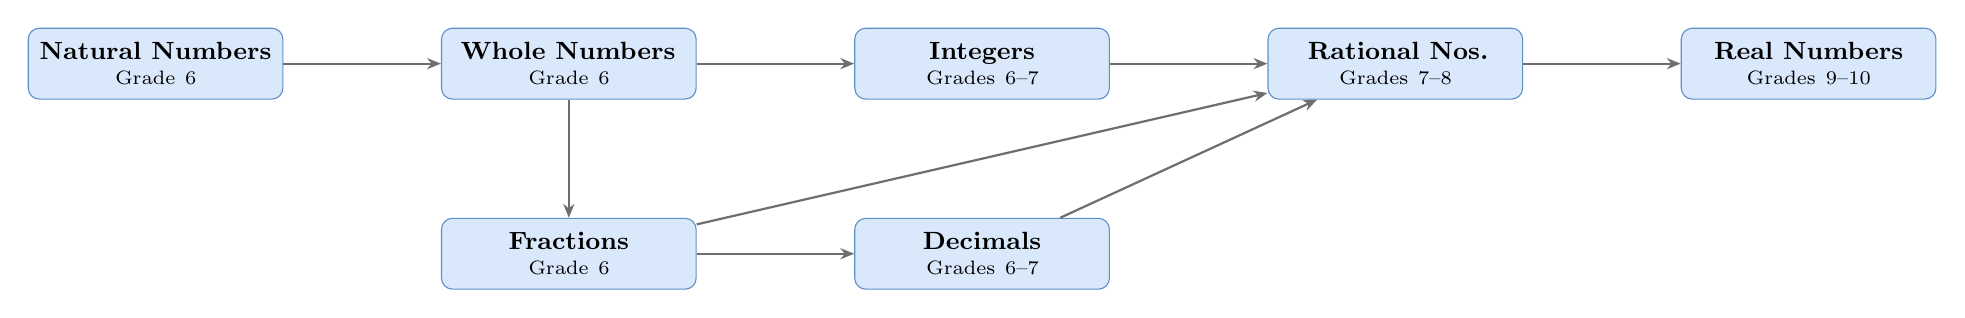
\begin{tikzpicture}[
  node distance = 1.25cm and 2.0cm,
  cnode/.style = {
    rectangle, draw=mainblue!70, fill=lightblue,
    rounded corners=4pt, text width=3.0cm,
    minimum height=0.9cm, align=center, font=\small\bfseries
  },
  arr/.style = {-{Stealth[length=5pt,width=4pt]}, thick, arrowgray}
]
  \node[cnode] (nat)   {Natural Numbers\\[-2pt]\scriptsize\normalfont Grade~6};
  \node[cnode, right=of nat]   (whole) {Whole Numbers\\[-2pt]\scriptsize\normalfont Grade~6};
  \node[cnode, right=of whole] (int)   {Integers\\[-2pt]\scriptsize\normalfont Grades~6--7};
  \node[cnode, below=1.5cm of whole] (frac) {Fractions\\[-2pt]\scriptsize\normalfont Grade~6};
  \node[cnode, right=of int]   (rat)   {Rational Nos.\\[-2pt]\scriptsize\normalfont Grades~7--8};
  \node[cnode, below=1.5cm of int]   (dec)  {Decimals\\[-2pt]\scriptsize\normalfont Grades~6--7};
  \node[cnode, right=of rat]   (real)  {Real Numbers\\[-2pt]\scriptsize\normalfont Grades~9--10};

  \draw[arr] (nat)   -- (whole);
  \draw[arr] (whole) -- (int);
  \draw[arr] (int)   -- (rat);
  \draw[arr] (whole) -- (frac);
  \draw[arr] (frac)  -- (rat);
  \draw[arr] (frac)  -- (dec);
  \draw[arr] (dec)   -- (rat);
  \draw[arr] (rat)   -- (real);
\end{tikzpicture}
\caption{A portion of the Number Systems subgraph.
         Each arrow means ``must understand before.''
         Concepts span multiple grade levels and the graph spans from Grade~6 through Grade~12.}
\label{fig:numsubgraph}
\end{figure}

\subsection{Manual Expert Curation}

A substantial part of the graph was built through manual curation rather than automated
generation alone.
Each concept was defined explicitly: its canonical name, the grades it covers,
which area it belongs to, its prerequisites, and a description of what the concept is.
The graph was rebuilt and re-validated computationally with every addition.

This was a deliberate choice.
Prerequisite relationships in mathematics and science can appear obvious but be wrong in
subtle ways that would mislead students.
An automated process can get the structure broadly right but misplace edges in ways that
matter educationally.
The manual curation pass produced a graph that is educationally sound throughout.

\subsection{Coverage: Mathematics and Science}

The knowledge graph covers the complete school curriculum for two subjects.

The \textbf{Mathematics graph} spans Grades~6 through~12 across eighteen mathematical areas:
Number Systems, Number Theory, Algebra, Geometry, Trigonometry, Coordinate Geometry,
Mensuration, Differential Calculus, Integral Calculus, Differential Equations, Vectors,
Three-Dimensional Geometry, Statistics, Probability, Combinatorics, Sequences and Series,
Complex Numbers, and Matrices and Determinants.
Concepts from different areas are linked wherever genuine prerequisites cross area boundaries:
trigonometric functions depend on both Geometry and Algebra;
calculus requires solid grounding in Algebra and Coordinate Geometry;
probability at the senior secondary level depends on combinatorics.
The longest prerequisite chain in the graph runs from the most foundational concepts
in Grade~6 through to advanced Grade~12 topics,
reflecting the genuine depth of the mathematical progression.

The \textbf{Science graph} covers Physics, Chemistry, and Biology across Grades~6 through~12.
Science presents different structural challenges than mathematics.
In Biology, many concepts are parallel rather than strictly sequential;
Physics and Chemistry have clearer prerequisite chains.
The science graph also includes cross-subject edges to mathematics,
because scientific reasoning often depends directly on mathematical tools.
``Newton's Second Law'' has a prerequisite link to ``Ratios and Proportions.''
``Electric Circuit Analysis'' links to ``Linear Equations.''
These connections mean a student can see not just the scientific prerequisites of a concept
but also the mathematical tools they will need.

Together, the two graphs represent everything a school student in India encounters
in Mathematics and Science from Grade~6 through Grade~12,
across all of the major curriculum boards.

%% ═══════════════════════════════════════════════════════════════════════════
\section{Content Generation}

\subsection{Grounding Explanations in the Textbooks}

Generating educational content purely from a language model's internal knowledge
is unreliable.
Models produce explanations that sound authoritative but contain subtle errors:
wrong formula applications, imprecise definitions, incorrect reasoning steps.
This is especially problematic in mathematics, where a single incorrect step
can make a derivation or proof entirely meaningless.

The solution is \emph{Retrieval-Augmented Generation (RAG)}.
Rather than relying on the model's parametric memory alone,
the system retrieves relevant passages from trusted reference material
and provides them as context when generating content.

The trusted reference material is the original NCERT textbooks.
All textbook content was processed into short passages and stored in a
\emph{vector database}, a database that supports semantic similarity search,
finding passages that are about the same idea as a query
rather than just sharing exact keywords.
When generating content for any concept, the system retrieves the most relevant textbook
passages for that concept and includes them in the generation prompt.
The model then writes an explanation grounded in the actual textbook material,
which greatly reduces the risk of invented or incorrect content compared to
the Phase~1 approach.

Equally important, the generation prompt includes brief summaries of all prerequisite
concepts.
This means every explanation naturally builds on what the student already knows,
uses the same terminology as related concept pages,
and can explicitly refer to prior knowledge.
Because all concepts are generated with the same prerequisite summaries,
the terminology is consistent across every related page;
the terminology drift problem from Phase~1 is resolved at the structural level,
not patched after the fact.

\subsection{Direct Multilingual Generation}

Phase~1 generated content in English and ran a separate translation pass.
Phase~2 eliminates translation entirely.

For each concept, content is generated in English, Hindi, Telugu, and Odia as four
parallel generation runs, all using the same RAG-assembled context.
For the Indic language runs, Sarvam~AI models are used.
These are large language models trained with a strong emphasis on Indian languages
and Indian educational content.

Rather than converting an English explanation to Hindi,
the Sarvam model generates the Hindi explanation from scratch using the retrieved
textbook passages and prerequisite summaries as context,
the same way a Hindi-speaking teacher would write an explanation,
not the way a translator would convert one.

This approach has a decisive advantage for terminology.
A model that generates in Hindi has a fixed internal vocabulary for mathematical
and scientific terms.
The Hindi term it uses for ``derivative'' will be the same on every concept page
it generates, because it is not making a fresh translation decision for each page.
It has learned what term is used for ``derivative'' in Hindi educational text
and applies it uniformly across the entire curriculum.
There is no independent random decision, no library version conflict,
and no post-processing needed to standardise terms.

Mathematical notation is embedded in the generated content as \LaTeX{} markup
by the model itself, in all four languages.
Because formulas are generated directly (not passed through a translation layer),
there is no possibility of corruption.
The same formula appears identically in the English, Hindi, Telugu, and Odia versions
of any concept page.

%% ═══════════════════════════════════════════════════════════════════════════
\section{The Web Platform}

\subsection{Architecture}

The platform consists of a Next.js web application and an API server,
with content stored in a cloud-hosted database.
Next.js is a web framework that supports both server-rendered and statically generated pages;
the platform uses static generation for concept pages wherever possible.

At build time, all concept pages are pre-rendered as static HTML.
When a student visits a concept page, the page is served immediately
with no database query or server computation required.
Static rendering produces fast load times on slower mobile connections,
which matters for students in areas where high-speed internet is not available.
All four language versions of every page are pre-rendered in the same way.

\subsection{Navigating the Graph}

The experience begins at a subject hub (Mathematics or Science).
The hub shows the areas the subject is divided into, with colour coding
that is used consistently throughout the interface.
Selecting a grade shows all concepts taught at that grade, grouped by area.

\begin{figure}[H]
\centering
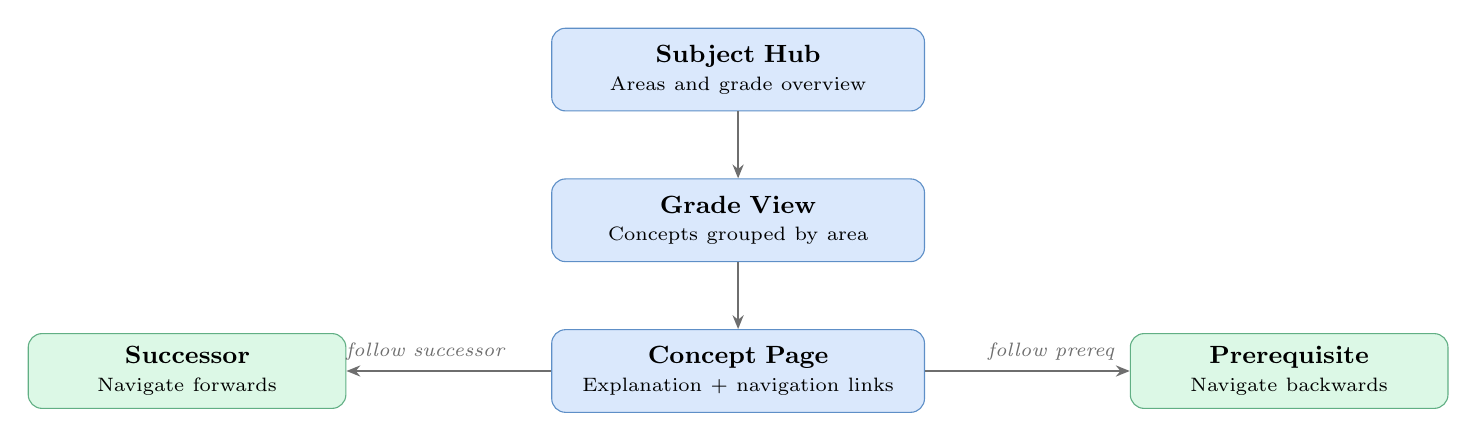
\begin{tikzpicture}[
  node distance = 0.85cm and 0.4cm,
  pnode/.style = {
    rectangle, draw=mainblue!70, fill=lightblue,
    rounded corners=5pt, text width=4.5cm,
    minimum height=1.05cm, align=center, font=\small
  },
  snode/.style = {
    rectangle, draw=nodegreen!70, fill=lightgreen,
    rounded corners=5pt, text width=3.8cm,
    minimum height=0.95cm, align=center, font=\small
  },
  arr/.style = {-{Stealth[length=5pt,width=4pt]}, thick, arrowgray}
]
  \node[pnode] (hub)     {\textbf{Subject Hub}\\[-1pt]\scriptsize\normalfont Areas and grade overview};
  \node[pnode, below=of hub]   (grade)   {\textbf{Grade View}\\[-1pt]\scriptsize\normalfont Concepts grouped by area};
  \node[pnode, below=of grade] (concept) {\textbf{Concept Page}\\[-1pt]\scriptsize\normalfont Explanation + navigation links};
  \node[snode, right=2.6cm of concept] (pre) {\textbf{Prerequisite}\\[-1pt]\scriptsize\normalfont Navigate backwards};
  \node[snode, left=2.6cm of concept]  (nxt) {\textbf{Successor}\\[-1pt]\scriptsize\normalfont Navigate forwards};

  \draw[arr] (hub)     -- (grade);
  \draw[arr] (grade)   -- (concept);
  \draw[arr] (concept.east) -- node[above,font=\scriptsize\itshape,text=arrowgray,xshift=0.3cm]{follow prereq} (pre.west);
  \draw[arr] (concept.west) -- node[above,font=\scriptsize\itshape,text=arrowgray,xshift=-0.3cm]{follow successor} (nxt.east);
\end{tikzpicture}
\caption{Navigation structure of the platform. From any concept page, a student
         can move backwards through prerequisites or forward through successors,
         in any of the four supported languages.}
\label{fig:nav}
\end{figure}

\subsection{The Concept Page}

The individual concept page is the heart of the platform.
A student arrives here either by browsing a grade view, following a link from a related concept,
or searching by name.
The page presents the following in a clean, readable layout:

\begin{itemize}[leftmargin=2em, itemsep=0.3em]

  \item \textbf{Area badge and grade context.}
    The concept's mathematical or scientific area is shown as a colour-coded badge.
    If the concept appears in multiple grades (a common situation, since foundational topics
    like ``Linear Equations'' are relevant across several years),
    all grade versions are linked, so a student can easily navigate to a more advanced
    or more introductory treatment of the same idea.

  \item \textbf{Description.}
    A one- or two-sentence overview of what the concept is and why it matters.

  \item \textbf{Prerequisites.}
    Every concept the student should have studied before arriving here,
    shown as clickable cards.
    Each card shows the prerequisite's name, its area, and the grade levels it covers.
    Clicking navigates directly to that concept's page.
    A student who is confused can follow prerequisite links backwards until they find
    the gap in their understanding.

  \item \textbf{The full explanation.}
    Generated by the content pipeline with textbook grounding and prerequisite context.
    Mathematical notation is rendered as properly typeset symbols.
    Explanations are written at the appropriate level for the grade:
    conversational and example-rich for lower grades,
    more rigorous and formally precise for upper secondary.

  \item \textbf{What this concept unlocks.}
    Concepts that become accessible after mastering this one,
    presented in the same style as prerequisites.
    A student who has mastered something can immediately see what it opens up next.

\end{itemize}

This structure is qualitatively different from anything based on textbook chapters.
A student struggling with ``Integration by Parts'' can follow prerequisite links backwards:
to ``Integration by Substitution,'' then ``Product Rule of Differentiation,''
then ``Limits and Continuity,'' and further back through the chain if needed.
They can trace exactly where the gap lies.
A student who has mastered a topic can follow the successor links forward and navigate
through the curriculum at their own pace without waiting for a chapter to tell them
what comes next.

\subsection{Language Selection and Mathematical Notation}

Every concept page is available in all four languages: English, Hindi, Telugu, and Odia.
A language selector switches the explanation text to the chosen language.
Navigation elements, concept names, and area labels remain consistent across all languages.
Mathematical notation is identical across all language versions
because it was generated alongside the language content, not translated from another version.

A student reading in Odia encounters an explanation that was written in Odia,
grounded in the same textbook material, using the standard Odia educational terminology
for every mathematical and scientific term that appears.
There is no residue of an English source text; the content is native to its language.

\subsection{Search}

A global search bar, accessible from any page, finds concepts by name, area, or description.
Typing a term returns all related concepts across grades and subjects,
each shown with its area and grade levels.
A student who remembers learning something about triangles but does not remember
which grade or chapter can search for it and find all relevant concept pages immediately.
Concepts that serve as natural starting points in a given grade (those with no prerequisites
at that level) are highlighted, guiding students who are beginning a new grade toward
where they should start.

%% ═══════════════════════════════════════════════════════════════════════════
\section{Discussion}

\subsection{What Phase~1 Taught Us}

The Phase~1 pipeline was built and run in full before being abandoned.
This was not wasted effort.
Running it produced concrete evidence of exactly what failed and why,
which made the design of Phase~2 well-grounded rather than speculative.

The five problems identified in Phase~1 (inconsistency from multiple generation,
absence of navigation, model hallucination, terminology drift, and structural redundancy)
all traced to a single root cause: the chapter section was the wrong abstraction.
Recognising this clearly, rather than patching around it, justified the substantial
effort of rebuilding from scratch.

\subsection{The Knowledge Graph as an Educational Artefact}

The knowledge graphs built in this project are not just data structures for the software system.
They are educational artefacts in their own right.

The process of building them required the project team to think carefully about
what every topic in the school curriculum actually depends on and what it enables.
Questions arose that textbooks never make explicit:
Does understanding inequalities require understanding equations first,
or can they be taught in parallel?
Is ``the Pythagorean Theorem'' a prerequisite for trigonometry,
or is it co-taught at the same point?
These questions have right answers, and working through them for every concept across
seven grades in two subjects produced a structure that has genuine educational value
beyond the software it supports.

The graph also revealed the cross-subject connections that curricula typically
leave implicit.
The mathematics a student needs for electromagnetism, for gas law calculations,
for genetics probability: these connections exist, and making them explicit in the graph
means the platform can surface them rather than leaving students to discover them by chance.

\subsection{Comparison with the Phase~1 Approach}

The fundamental difference between the two phases is one of design philosophy.

Phase~1 optimised for the \emph{production} of content: extract, generate, translate, store.
The goal was to have a page for every textbook section.
Phase~2 optimises for the \emph{coherence} of content: define once, generate with context,
produce natively in each language.
The goal is to have one authoritative, connected page for every concept.

Phase~1 produced more raw pages faster.
Phase~2 produced less content but content that is correct, navigable, consistent,
and educationally grounded.
For a platform students are meant to actually use and trust for a subject as
exacting as mathematics, the Phase~2 approach is the only defensible one.

%% ═══════════════════════════════════════════════════════════════════════════
\section{Conclusion}

This project built a multilingual educational platform for Indian school students
that does not exist elsewhere in free form: concept-structured, multi-board,
covering Mathematics and Science for Grades~6 through~12,
with content generated directly in English, Hindi, Telugu, and Odia.

The path involved building a first version, identifying its failures precisely,
understanding those failures as design problems rather than implementation bugs,
and redesigning from scratch around the correct abstraction.
The knowledge graph, the core artifact of Phase~2, is the result of that redesign.

The platform gives a student something no digitised textbook can:
a map of what they are trying to learn.
Every concept they encounter has a page that shows them what they need to know before it
and where it leads afterward.
They can follow that map in any direction, in their own language,
with explanations grounded in the textbooks their curriculum uses.

The result is a tool that treats learning as the interconnected, cumulative, direction-having
activity it actually is, rather than as a flat sequence of chapters to be completed
in order.

\end{document}
